\documentclass{report}

\usepackage[textwidth=16cm, textheight=24cm]{geometry}
% Packages for special characters and symbols
\usepackage[utf8]{inputenc}
\usepackage[T1]{fontenc}
\usepackage{amsmath, amssymb, amsthm}

% Package for hyperlinks
\usepackage{hyperref}

% Package for graphics
\usepackage{graphicx, caption}
\usepackage{fancyhdr} % For fancy headers and footers
\usepackage[export]{adjustbox}
\usepackage{subcaption}
\usepackage{multicol}
\usepackage{float}
\usepackage{listings}
\usepackage{dirtree}

% Package for better tables
\usepackage{booktabs}
\usepackage{xepersian}





% Page dimensions and margin settings
\geometry{
  top=0.5cm,
%   left=3cm,
  headheight=40pt, % Adjust the header height
  headsep=10pt, % Separation between header and text
  includeheadfoot
}

% Path to your logo
\newcommand{\headerlogo}{images/Logo.png}

% Header and footer configuration
\pagestyle{fancy}
\fancyhf{} % Clear header and footer
\fancyhead[R]{\includegraphics[height=40pt]{\headerlogo}} % Logo on the Left of the header
\fancyfoot[C]{\thepage} % Page number at the center of the footer

% Ensure the header and footer lines are removed
\renewcommand{\headrulewidth}{0.4pt}
\renewcommand{\footrulewidth}{0pt}





% \setlatintextfont{Times New Roman}
% \settextfont{Yas.ttf}
\settextfont[
BoldFont=Yas Bd.TTF]{Yas.TTF}
% Set the title, author, and date
\title{گزارش پروژه پنجم علوم اعصاب محاسباتی}
\author{امیرحسین انتظاری}
\date{\today}

% Begin document
\begin{document}
\begin{figure}
    \centering 
\includegraphics[height=3cm]{images/Logo.png}
\end{figure}
% Redefine chaptername
\renewcommand{\chaptername}{بخش}
\newpage
% Create the title
\maketitle
\newpage
% Create a table of contents
\tableofcontents
% Separate the table of contents from the next content with a new page
% \clearpage

\newgeometry{textwidth=13cm,textheight=22cm}
    \begin{abstract}
        هدف از این پروژه بررسی و شبیه‌سازی پردازش تصاویر در نواحی اولیه قشر بینایی است. این پژوهش شامل مدلسازی نحوه پردازش و تفسیر محرک‌های بصری توسط سیستم بینایی انسان می‌شود. در این پروژه، از فیلترهای تفاضل گاوسی 
        (DoG) 
        و گبور استفاده شده است تا مکانیسم‌های پردازشی شبکیه و قشر بینایی 
        V1 
        را شبیه‌سازی کنند.

        فیلترهای 
        DoG \footnote{\lr{Difference of Gaussian}}
        به تقلید از میدان‌های گیرنده سلول‌های گانگلیونی شبکیه و لوب زانویی جانبی 
        (LGN \footnote{\lr{Lateral geniculate nucleus}}) 
        به منظور تشخیص لبه‌ها و کنتراست محلی استفاده می‌شوند. فیلترهای گبور نیز به دلیل توانایی‌شان در شبیه‌سازی میدان‌های گیرنده انتخابی جهت‌گیری در قشر بینایی اولیه (V1)، 
        برای تحلیل لبه‌ها و بافت‌ها به کار رفته‌اند.
        
        همچنین، پروژه به بررسی کدگذاری عصبی ضربه‌ای 
        (SNN\footnote{\lr{Spiking Neural Network}}) 
        بر اساس خروجی فیلترها پرداخته و نتایج نشان داده‌اند که پیش‌پردازش با فیلترهای DoG و گبور می‌تواند ویژگی‌های بصری مهم را برجسته کند و بهبود‌هایی در کدگذاری و پردازش عصبی ایجاد کند.
        \end{abstract}
\restoregeometry


\newpage
\chapter{چگونگی پردازش تصاویر در نواحی اولیه قشر بینایی}
    \section{مقدمه}
        یکی از جنبه های مهم علوم اعصاب محاسباتی شامل مدل سازی نحوه تفسیر و پردازش محرک های بصری توسط سیستم بینایی است. مراحل اولیه پردازش بصری در شبکیه و قشر بینایی اولیه 
        (V1) 
        رخ می دهد، جایی که اطلاعات بصری پیچیده ابتدا به الگوهای معنی دار کدگشایی می شوند. این پروژه بر شبیه سازی مکانیسم های پردازش تصویر لایه اول مسیر بصری با استفاده از فیلترهای تفاوت گاوسی 
        (DoG)\footnote{\lr{Difference of Gaussian}}
        و فیلترهای گبور
        \footnote{Gabor}
        تمرکز دارد.

        شبکیه و مسیر بینایی اولیه به طور گسترده مورد مطالعه قرار گرفته اند تا بفهمند که چگونه ورودی های بصری خام به نمایش های ساختاری تبدیل می شوند. در این مرحله، نورون ها میدان های دریافتی را نشان می دهند که به طور انتخابی به ویژگی های بصری مختلف مانند لبه ها، جهت گیری ها و فرکانس های فضایی پاسخ می دهند. دو مدل برجسته که این ویژگی‌ها را نشان می‌دهند، فیلتر تفاضل گاوسی 
        (DoG) 
        و فیلترهای گبور هستند.
        
        فیلترهای 
        DoG 
        برای مدل‌سازی میدان‌های گیرنده در اطراف سلول‌های گانگلیونی شبکیه و نورون‌های هسته ژنیکوله جانبی 
        (LGN) 
        استفاده می‌شوند. این فیلترها با برجسته کردن مناطقی که شدت تغییر سریع دارند، کنتراست را برجسته می‌کنند و به طور موثر لبه‌ها و کنتراست‌های محلی را در صحنه بصری تشخیص می‌دهند. فیلترهای 
        DoG 
        با تقلید از سازمان محیطی مرکز، راه بیولوژیکی قابل قبولی را برای پیش پردازش اطلاعات بصری، کاهش افزونگی و افزایش ویژگی های برجسته ارائه می دهند.
        
        از سوی دیگر، فیلترهای گبور در مدل‌سازی میدان‌های گیرنده انتخابی جهت‌گیری موجود در قشر بینایی اولیه 
        (V1) 
        ابزاری هستند. این فیلترها می‌توانند جهت‌گیری‌ها و فرکانس‌های فضایی خاص را در ورودی بصری شناسایی کنند، که دقیقاً با ویژگی‌های تنظیم سلول‌های ساده در 
        V1 
        مطابقت دارد. بنابراین، فیلترهای گبور می‌توانند ماهیت چگونگی پردازش لبه‌ها و بافت‌ها توسط قشر بینایی را به تصویر بکشند و در مراحل اولیه ادراک بصری و تشخیص الگوی نقش داشته باشند.
        
        در این پروژه، فیلترهای 
        DoG و Gabor 
        را برای شبیه سازی مراحل اولیه پردازش بصری پیاده سازی کردیم. پیاده سازی شامل ایجاد این فیلترها، اعمال آنها بر روی تصاویر ورودی مختلف و تجزیه و تحلیل خروجی های آنها برای درک نقش آنها در پردازش بصری است.
        
        با بررسی قابلیت‌های فیلترهای 
        DoG و Gabor، 
        این مطالعه با هدف پر کردن شکاف بین بینایی بیولوژیکی و مدل‌های محاسباتی، ارائه درک جامعی از فرآیندهای اساسی زیربنای ادراک بصری است. در بخش‌های بعدی روش‌شناسی، پیاده‌سازی و نتایج به‌کارگیری این فیلترها برای محرک‌های بصری را به تفصیل شرح داده می‌شود.
    \section{فیلتر تفاضل گاوسی}
    اولین لایه مسیر بینایی که به شبکیه معروف است، نقش مهمی در مراحل اولیه پردازش تصویر دارد. این لایه وظیفه جذب نور و تبدیل آن به سیگنال های عصبی را بر عهده دارد که سپس برای تفسیر بیشتر به مغز منتقل می شود. یکی از جنبه های کلیدی این پردازش شامل تمایز اطلاعات بصری، به ویژه تشخیص لبه ها و تضادها در میدان بینایی است. یکی از مدل‌های محاسباتی مؤثر که این فرآیند بیولوژیکی را تقلید می‌کند، فیلتر تفاوت گاوسی 
    (DoG) 
    است.

    فیلتر 
    DoG 
    از میدان‌های گیرنده سلول‌های گانگلیونی شبکیه الهام گرفته شده است که برای تشخیص لبه و افزایش کنتراست در سیستم بینایی ضروری است. سلول های گانگلیونی در شبکیه، نورون های تخصصی هستند که اطلاعات بصری را قبل از ارسال به مغز پردازش می کنند. این سلول‌ها دارای میدان‌های گیرنده هستند که شامل یک ناحیه مرکزی است که توسط نور برانگیخته یا مهار می‌شود و یک ناحیه اطراف آن که واکنش مخالف را نشان می‌دهد. این مکانیسم به سلول‌های گانگلیونی اجازه می‌دهد لبه‌ها و تغییرات شدت نور را تشخیص دهند و نقش مهمی در ادراک بصری ایفا کنند.

    فیلتر 
    DoG 
    به طور ریاضی مکانیسم سلول‌های گانگلیونی را با کم کردن یک تاری گاوسی وسیع‌تر 
    (نماینده اطراف) 
    از یک تاری گاوسی باریکتر 
    (نماینده مرکز) 
    شبیه‌سازی می‌کند. این تفریق لبه‌ها و جزئیات ظریف ورودی بصری را افزایش می‌دهد، شبیه به پردازش انجام شده توسط سلول‌های گانگلیونی شبکیه. با تقلید از رفتار این سلول ها، فیلترهای 
    DoG 
    روشی قوی برای برجسته کردن مناطق با کنتراست بالا و سرکوب مناطق یکنواخت در یک تصویر ارائه می کنند.
    (شکل \ref{fig:part1-ganglion-cells-schematic})
    \begin{figure}[!ht]
        \centering
        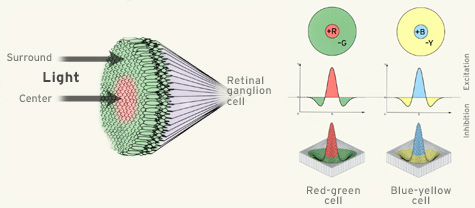
\includegraphics[width=0.8\textwidth]{images/ganglion-cells.jpg} 
        \captionsetup{width=.8\linewidth}
        \caption{\textbf{شمای کلی از سلول های گانگلیونی و ارتباط آن ها با فیلتر 
        DoG.}}
        \label{fig:part1-ganglion-cells-schematic}
    \end{figure}
    در این بخش پروژه، فیلترهای 
    DoG 
    را برای مدل‌سازی پردازش تصویری که در لایه اول مسیر بصری رخ می‌دهد، پیاده‌سازی کردیم. هدف اجرای ما تکرار عملکرد بیولوژیکی سلول‌های گانگلیونی شبکیه است و بینش‌هایی در مورد اینکه چگونه سیستم بینایی انسان به طور موثر اطلاعات بصری را شناسایی و پردازش می‌کند، ارائه می‌کند. از طریق این رویکرد محاسباتی، ما اثربخشی فیلترهای 
    DoG 
    را در بهبود ویژگی‌های تصویر بررسی می‌کنیم و زمینه را برای تحقیقات بیشتر در مورد مکانیسم‌های پردازش بصری پیچیده‌تر فراهم می‌کنیم.

    \subsection{دیدگاه ریاضی}
        در علم تصویربرداری، تفاوت گاوسی ها 
        (DoG) 
        یک الگوریتم بهبود ویژگی است که شامل تفریق یک نسخه تار گاوسی یک تصویر اصلی از نسخه دیگر، کمتر تار شده اصلی است. در مورد ساده تصاویر مقیاس خاکستری، تصاویر تار با انحراف تصاویر اصلی در مقیاس خاکستری با هسته
        \footnote{kernel}
        های گاوسی با عرض متفاوت 
        (انحرافات استاندارد) 
        به دست می آیند. محو کردن یک تصویر با استفاده از هسته گاوسی فقط اطلاعات مکانی با فرکانس بالا را سرکوب می کند. با کم کردن یک تصویر از تصویر دیگر، اطلاعات فضایی که بین محدوده فرکانس‌هایی که در دو تصویر تار حفظ می‌شوند، حفظ می‌شود. بنابراین، 
        DoG 
        یک فیلتر  میان‌گذر فضایی است که فرکانس‌های تصویر اصلی مقیاس خاکستری را که دور از مرکز هستند، کاهش می‌دهد.
 
        $\Phi_t : \mathbb{R}^n \rightarrow \mathbb{R}$ 
        را به عنوان تابع گاوسی شعاعی 
        $\Phi_t(x) = \mathcal{N}(x|0, t)$ 
        با میانگین 
        $0$ 
        و واریانس 
        $t$، 
        یعنی، تابع گاوسی چندمتغیره 
        $\Phi_t(x) = \mathcal{N}(x|0, tI)$ 
        با میانگین 
        $0$ 
        و کوواریانس 
        $tI$ 
        در نظر بگیرید. به طور صریح‌تر، داریم
        \[
        \Phi_t(x) = \frac{1}{(2\pi t)^{n/2}} e^{-\frac{|x|^2}{2t}}.
        \]
        تفاوت گاوسی‌ها با واریانس‌های 
        $t_1 < t_2$ 
        تابع هسته
        \[
        K_{t_1, t_2} = \Phi_{t_1} - \Phi_{t_2}
        \]
        است که با تفریق گاوسی با واریانس بالاتر از گاوسی با واریانس کمتر به دست می‌آید. تفاوت عملگر گاوسی همان عملگر کانولوشن مرتبط با این تابع هسته‌ای است. شکل کلی این فیلتر در شکل 
        \ref{fig:part1-DoG}
        نشان داده شده است.
        \begin{figure}[!ht]
            \centering
            \begin{subfigure}[b]{0.4\textwidth}
                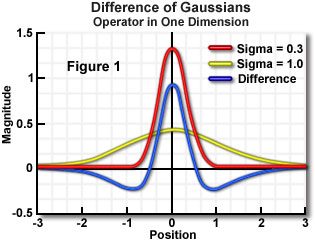
\includegraphics[width=\textwidth]{images/DoG-filter.jpg}
                \caption{شکل کلی نحوه انجام تفاضل گاوسی}
                \label{fig:part1-DoG-filter}
            \end{subfigure}
            \hfill % optional; use for aligning images side by side
            \begin{subfigure}[b]{0.4\textwidth}
                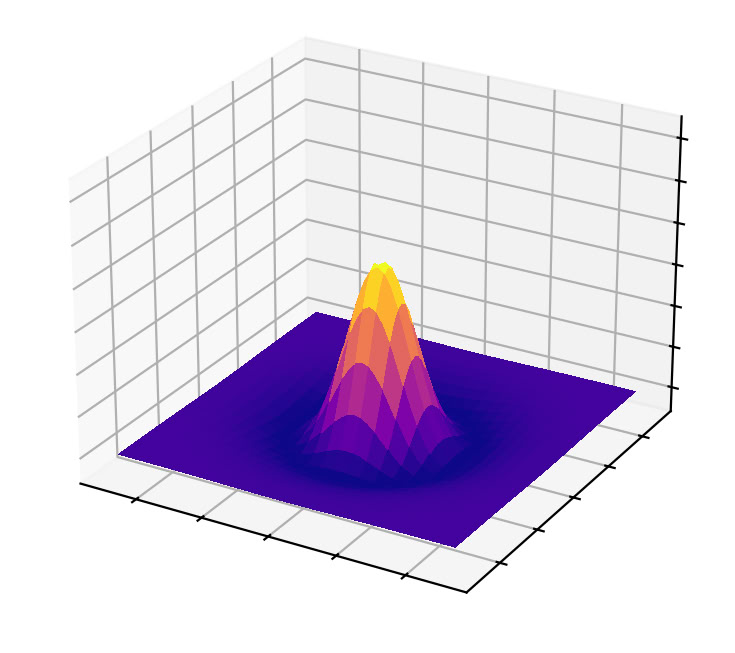
\includegraphics[width=\textwidth]{images/DoG-3d.jpg}
                \caption{شکل ۳ بعدی تفاضل گاوسی}
                \label{fig:part1-DoG-3d}
            \end{subfigure}
            \caption{ تفاضل گاوسی (DoG)}
            \label{fig:part1-DoG}
        \end{figure}
        \subsection{تاثیر پارامتر ها}
            حال در این قسمت تاثیر هر یک از پارامتر ها در فیلتر ها را بررسی می‌کنیم. ما بر نقش دو پارامتر کلیدی تمرکز می کنیم: انحرافات استاندارد دو فیلتر گاوسی اعمال شده. تأثیر آن‌ها بر نتیجه فرآیند فیلتر کردن 
            DoG 
            از طریق مجموعه‌ای از آزمایش‌های طراحی‌شده به‌صورت روش‌مند تحلیل می‌شود و نشان می‌دهد که چگونه تغییرات در این پارامترها بر حساسیت و ویژگی تشخیص لبه تأثیر می‌گذارد.(شکل \ref{fig:part1-DoG-Kernel})

            \begin{figure}[!ht]
                \centering
                \includegraphics[width=\textwidth]{plots/part1-DoG-Kernel.pdf} 
                \captionsetup{width=.9\linewidth}
                \caption{\textbf{مقایسه تاثیر پارامتر های فیلتر DoG.} 
                این شکل سه فیلتر 
                DoG 
                را با مقادیر سیگما متفاوت نشان می‌دهد تا تأثیر آنها بر قابلیت‌های تشخیص لبه را نشان دهد. شکل بالایی یک هسته با $\sigma_1=3 $و $\sigma_2=6 $
                را نشان می دهد که برای تشخیص جزئیات بسیار ایده آل است. شکل میانی با 
                $\sigma_1=4 $و $\sigma_2=8$ 
                پاسخ وسیع تری را برای لبه های برجسته نشان می دهد. شکل پایین دارای یک هسته خارج از مرکز با 
                $\sigma_1=6$ و $\sigma_2=3$ 
                است که حساسیت به ویژگی های جهت را افزایش می دهد. هر فیلتر به صورت سه بعدی نیز برای درک بهتر آمده است.}
                \label{fig:part1-DoG-Kernel}
            \end{figure}
        \subsection{خروجی تصویر پس از اعمال فیلتر DoG}
            حال در این بخش، یک فیلتر 
            DoG 
            را روی یک تصویر نمونه اعمال کرده و خروجی آن را نشان می‌دهیم. برای اینکار، یک تصویر نمونه که از مخزن دانشگاه واترلو 
            \footnote{\href{https://links.uwaterloo.ca/Repository.html}{https://links.uwaterloo.ca/Repository.html}}
            انتخاب کرده و فیلتر 
            DoG 
            را با اندازه های مختلف و همچنین دو نسخه 
            on-center 
            و 
            off-center 
            را روی آن هم‌گشت
            \footnote{Convolution}
            می‌کنیم. 

            شکل
            \ref{fig:part1-DoG-on-image}
            کاربرد فیلتر تفاوت گوسی ها 
            (DoG) 
            را بر روی یک تصویر نمونه نشان می دهد، که اثرات آن را با مقادیر مختلف سیگما و کنتراست نسخه های 
            on-center
            و 
            off-center
            نشان می دهد.

            تصویر ورودی که در بالا سمت چپ نشان داده شده است، به عنوان محرک بصری اصلی برای فرآیندهای فیلتر بعدی عمل می کند. در مجاورت این تصویر، هسته 
            DoG 
            نشان داده شده است که با تفریق دو تابع گاوسی با انحرافات استاندارد مختلف 
            (سیگما) 
            ساخته شده است. این هسته برای شبیه سازی خواص میدان پذیرای سلول های گانگلیونی شبکیه است.

            در ردیف وسط، خروجی فیلتر 
            DoG 
            با نسخه
            on-center
            ارائه شده است. این نسخه بر نواحی تأکید دارد که بخش مرکزی میدان گیرنده توسط نور برانگیخته می شود و به طور مؤثر لبه ها و جزئیات ظریف درون تصویر را برجسته می کند. مقادیر مختلف سیگما برای نشان دادن اینکه چگونه گستردگی توابع گاوسی بر تشخیص لبه‌ها تأثیر می‌گذارد نیز در ردیف پایین اعمال می‌شود، با سیگماهای کوچکتر که جزئیات ریزتر را افزایش می‌دهند و سیگماهای بزرگ‌تر ساختارهای وسیع‌تری را جذب می‌کنند.

            ستون اول از سمت راست خروجی 
            off-center
            فیلتر 
            DoG 
            را نشان می دهد. در اینجا، فیلتر تنظیم شده است تا مناطقی را که بخش مرکزی میدان گیرنده توسط نور مهار می شود، بهبود بخشد، و در نتیجه تضاد تکمیلی با خروجی در مرکز ایجاد می کند. تغییر در مقادیر سیگما به طور مشابه بر سطح جزئیات و میزان تشخیص لبه تأثیر می‌گذارد و انعطاف‌پذیری فیلتر 
            DoG 
            را در مدل‌سازی جنبه‌های مختلف پردازش بصری نشان می‌دهد.

            \begin{figure}[!ht]
                \centering
                \includegraphics[width=0.95\textwidth]{plots/part1-DoG-convolution.pdf} 
                \captionsetup{width=.9\linewidth}
                \caption{\textbf{کاربرد تفاضل فیلتر گاوسی 
                (DoG) 
                روی یک تصویر نمونه.} 
                شکل، فرآیند و اثرات اعمال فیلتر 
                DoG 
                بر روی یک تصویر ورودی را نشان می دهد. 
                (ستون اول از سمت چپ) 
                تصویر ورودی اصلی که برای فیلتر کردن استفاده می شود. 
                (ستون دوم از سمت چپ) 
                هسته 
                DoG 
                با تفریق دو تابع گاوسی با انحرافات استاندارد مختلف (سیگما) 
                ایجاد شده است. 
                (ستون سوم از سمت چپ) 
                خروجی فیلتر 
                DoG 
                نسخه 
                on-center، 
                برجسته کردن لبه ها و جزئیات دقیق. مقادیر مختلف سیگما تأثیر بر تشخیص لبه و افزایش جزئیات را نشان می دهد. 
                (ستون جهارم از سمت چپ) 
                خروجی فیلتر 
                DoG 
                با نسخه
                off-center
                ، با تاکید بر مناطقی که مرکز توسط نور مهار می شود، و تضاد مکملی را با خروجی در مرکز نشان می دهد. تغییرات در مقادیر سیگما نشان داده شده است که انعطاف‌پذیری فیلتر 
                DoG 
                را در مدل‌سازی جنبه‌های مختلف پردازش بصری منعکس می‌کند.
                همانطور که مشاهده می‌کنیم، هر چه مقدار سیگما کوچکتر باشد، لبه های استخراج شده از تصویر نیز نازک تر است. با بزرگتر شدن این مقادیر در ستون دوم، تصویر حاصل نیز دارای خطوطی با ضخامت بیشتر می‌شود. }
                \label{fig:part1-DoG-on-image}
            \end{figure}

    \clearpage
    \section{فیلتر گبور}
        فیلترهای گبور ابزارهای محاسباتی هستند که به طور گسترده به دلیل توانایی آنها در شبیه سازی خواص میدان پذیری نورون ها در قشر بینایی اولیه 
        (V1) 
        شناخته شده است. این فیلترها که به نام دنیس گبور، که آنها را در سال 1946 معرفی کرد، نامگذاری شده‌اند، از آن زمان به بعد در درک چگونگی تفسیر اطلاعات بصری توسط مغز یکپارچه شده‌اند.

        فیلترهای گبور با توانایی آنها در گرفتن مکان یابی فضایی، انتخاب جهت گیری و تنظیم فرکانس فضایی مشخص می شوند، ویژگی هایی که بسیار با الگوهای پاسخ سلول های ساده در 
        V1 
        سازگار است. هر فیلتر گبور در اصل یک موج صفحه سینوسی است که توسط یک پوشش گاوسی ماژوله شده است.
        (گویی فیلتر 
        DoG 
        در یکی از محور های افقی خود کشیده شده است.
        شکل \ref{fig:part1-Gabor})
        این ترکیب به فیلتر اجازه می‌دهد تا به فرکانس‌ها و جهت‌گیری‌های فضایی خاص پاسخ دهد و آن را به ابزاری مؤثر برای تشخیص لبه، تحلیل بافت و استخراج ویژگی در تصاویر تبدیل می‌کند.
        
        از نظر ریاضی، یک فیلتر گبور را می توان به عنوان یک تابع نمایی پیچیده ضرب در یک تابع گاوس توصیف کرد. مولفه سینوسی لبه ها و خطوط را در یک جهت و مقیاس خاص تشخیص می دهد، در حالی که مولفه گاوسی با محدود کردن پاسخ فیلتر به یک منطقه محلی از تصویر، محلی سازی فضایی را تضمین می کند. نتیجه مجموعه‌ای از فیلترها است که هر کدام با جهت‌گیری‌ها و فرکانس‌های فضایی متفاوت تنظیم شده‌اند و طیف متنوعی از میدان‌های دریافتی موجود در قشر بینایی را تقلید می‌کنند.
        
        در این پروژه فیلترهای گبور را برای بررسی نقش آنها در پردازش بصری اولیه پیاده سازی کردیم. با اعمال این فیلترها بر روی یک سری از تصاویر، ما بررسی کردیم که چگونه آنها ویژگی های بصری خاص را افزایش می دهند و به درک کلی محرک بصری کمک می کنند.
        
        از طریق این کاوش، هدف ما نشان دادن اثربخشی فیلترهای گبور در گرفتن اطلاعات بصری ضروری و برجسته کردن اهمیت آنها در بینش بیولوژیکی و کاربردهای تکنولوژیکی است. بخش‌های بعدی به جزئیات فنی اجرای فیلتر گبور پرداخته می‌شود، نتایج اعمال این فیلترها را برای محرک‌های بصری مختلف ارائه می‌شود و مفاهیم آنها را برای درک ما از پردازش بصری مورد بحث قرار داده می‌شود.

        \begin{figure}[!ht]
            \centering
            \begin{subfigure}[b]{0.3\textwidth}
                
\includegraphics[width=\textwidth]{images/Gabor-2d.png}
                \caption{شکل ۲ بعدی فیلتر گبور}
                \label{fig:part1-Gabor-2d}
            \end{subfigure}
            \hfill % optional; use for aligning images side by side
            \begin{subfigure}[b]{0.5\textwidth}
                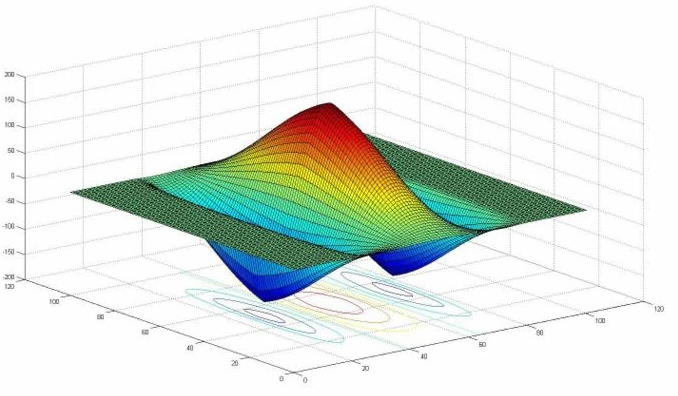
\includegraphics[width=\textwidth]{images/Gabor-3d.jpg}
                \caption{شکل ۳ بعدی فیلتر گبور}
                \label{fig:part1-Gabor-3d}
            \end{subfigure}
            \caption{فیلتر گبور}
            \label{fig:part1-Gabor}
        \end{figure}
        \subsection{دیدگاه ریاضی}
        فیلترهای گبور از نظر ریاضی در توابع پیچیده ای که امواج سینوسی را با پوشش های گاوسی ترکیب می کنند، پایه گذاری می شوند. این ساختار منحصربه‌فرد به آن‌ها اجازه می‌دهد هم فرکانس و هم اطلاعات مکانی را ضبط کنند، و آنها را برای مدل‌سازی پردازش بصری در مغز مناسب می‌سازد. در این بخش، فرمول ریاضی فیلترهای گبور و نحوه استفاده از آنها در وظایف پردازش تصویر را بررسی خواهیم کرد.
        
            \subsubsection*{تابع گبور}
            
            یک فیلتر گبور توسط یک تابع نمایی پیچیده که توسط یک تابع گاوسی مدوله شده است، تعریف می شود. شکل کلی فیلتر گبور دو بعدی را می توان به صورت زیر بیان کرد:
            
            \[ g(x، y؛ \lambda، \theta، \psi، \sigma، \gamma) = \exp \left( -\frac{x'^2 + \gamma^2 y'^2}{2\ sigma^2} \right) \exp \left( i \left( 2\pi \frac{x'}{\lambda} + \psi \right) \right) \]
            
            به طوری که:
            
            \[ x' = x \cos \theta + y \sin \theta \]
            \[ y' = -x \sin \theta + y \cos \theta \]
            
            در این معادله:
            \begin{itemize}
                \item  $\lambda$ (طول موج) فرکانس فضایی موج سینوسی را کنترل می کند.
                    \item  $\theta$  (جهت) جهت فیلتر را نشان می دهد.
                \item  $\psi$ (تغییر فاز) تغییر فاز تابع سینوسی را تعیین می کند.
                \item  $\sigma$ (انحراف معیار) پهنای گاوسی را مشخص می کند.
                \item  $\omega$ (نسبت ابعاد) بیضی بودن تابع گاوسی را تعریف می کند.
            \end{itemize}
            
            \subsubsection*{بخش های حقیقی و موهومی}
            
            یک فیلتر گبور را می توان به بخش های حقیقی و موهومی خود، مطابق با اجزای کسینوس و سینوسی تابع سینوسی، جدا کرد:
            
            \textbf{قسمت حقیقی:}
            \[ g_{\text{real}}(x, y؛ \lambda, \theta, \psi, \sigma, \gamma) = \exp \left( -\frac{x'^2 + \gamma^2 y '^2}{2\sigma^2} \right) \cos \left( 2\pi \frac{x'}{\lambda} + \psi \right) \]
            
            \textbf{قسمت موهومی:}
            \[ g_{\text{imag}}(x, y؛ \lambda, \theta, \psi, \sigma, \gamma) = \exp \left( -\frac{x'^2 + \gamma^2 y '^2}{2\sigma^2} \right) \sin \left( 2\pi \frac{x'}{\lambda} + \psi \right) \]
            
            این اجزا امکان جداسازی پاسخ فیلتر را به فازهای زوج و فرد فراهم می کند و تجزیه و تحلیل جامع تری از ویژگی های تصویر ارائه می دهد.
            
            در نتیجه، فرمول ریاضی فیلترهای گبور شامل ترکیبی از توابع گاوسی و سینوسی است که به آنها امکان می دهد هم اطلاعات مکانی و هم اطلاعات فرکانسی را ضبط کنند. با تنظیم پارامترها، این فیلترها را می توان برای تشخیص جهت گیری ها و مقیاس های مختلف تنظیم کرد و آنها را به ابزاری قدرتمند برای تجزیه و تحلیل تصویر و مدل سازی مکانیسم های پردازش بصری در مغز تبدیل کرد.
        \subsection{تاثیر پارامتر ها}
            حال در این قسمت، تاثیر هر یک از پارامتر ها در فیلتر ها را بررسی می‌کنیم. وابستگی پارامتری این فیلتر و تأثیراتی که این پارامترها بر پاسخ فیلتر دارند را مشخیص می‌کنیم. این پیاده‌سازی با تمرکز بر پارامترهای کلیدی مورد بحث قرار می‌گیرد: اندازه فیلتر، طول موج 
            ($\lambda$)، 
            جهت ($\theta$)، 
            انحراف استاندارد ($\sigma$)، 
            نسبت ابعاد ($\gamma$)، 
            و اندازه گام. هر پارامتر از طریق یک سری آزمایش های کنترل شده طراحی شده برای روشن کردن اثرات فردی آنها بر ویژگی های فیلتر حاصل بررسی می شود.

            نتایج بصری از این آزمایش‌ها برای نشان دادن اثرات ملموس تغییرات پارامترها، ارائه بینش‌هایی در مورد چگونگی تنظیم هر پارامتر برای بهینه‌سازی عملکرد فیلتر برای کاربردهای خاص ارائه شده است.(شکل \ref{fig:part1-Gabor-Kernel})
            \begin{figure}[!ht]
                \centering
                \includegraphics[width=0.9\textwidth]{plots/part1-Gabor-Kernel.pdf} 
                \captionsetup{width=.9\linewidth}
                \caption{\textbf{مقایسه تاثیر پارامتر های فیلتر گبور.} در این شکل، تاثیر هر یک از پارامتر های 
                اندازه فیلتر، طول موج 
                ($\lambda$)، 
                جهت ($\theta$)، 
                انحراف استاندارد ($\sigma$)، 
                نسبت ابعاد ($\gamma$)، 
                بررسی شده است. 
                هر نمودار تغییرات فرکانس مکانی و ویژگی‌های جهت‌گیری فیلتر را نشان می‌دهد و مشخص می‌کند که چگونه مقداردهی پارامتر می‌تواند پاسخ فیلتر را به ویژگی‌های خاص در برنامه‌های پردازش تصویر تنظیم کند. نمایش‌های سه‌بعدی در ردیف پایین، نیز برای درک عمیق تر این تاثیرات آمده است.}
                \label{fig:part1-Gabor-Kernel}
            \end{figure}


        \subsection{خروجی تصویر پس از اعمال فیلتر گبور}
            در این بخش مشابه قسمت قبل یک فیلتر گبور را روی یک تصویر نمونه هم‌گشت(convolve)
            می‌کنیم و خروجی آن را نمایش می‌دهیم.
            برای اینکار، تصویری که در بخش قبل به عنوان نمونه انتخاب کردیم را در اینجا نیز آورده و فیلتر گبور را با دو نسخه 
            off-center و on-center 
            روی آن اعمال می‌کنیم. شکل 
            \ref{fig:part1-Gabor-convolution}
            تصویر ورودی، هسته گبور و تصاویر فیلتر شده حاصل را نشان می دهد.

            مطابق قسمت قبل، شکل بالا سمت چپ، تصویر نمونه را نشان می‌دهد.
            سپس هسته گبور مورد استفاده برای کانولوشن نمایش داده می شود. این کرنل با پارامترهایی مانند طول موج، جهت گیری، فاصله فاز و نسبت ابعاد مشخص می شود که نحوه تعامل فیلتر با تصویر ورودی را مشخص می کند. نمایش بصری هسته گبور جهت گیری و ویژگی های فرکانس آن را برجسته می کند و نمای واضحی از عملکرد فیلتر ارائه می دهد.
            
            سپس شکل خروجی فیلتر گبور 
            on-center
            اعمال شده روی تصویر ورودی را نشان می دهد. در این نسخه، فیلتر ویژگی‌های مرکزی تصویر را افزایش می‌دهد و مناطقی را برجسته می‌کند که با جهت‌گیری و ویژگی‌های فرکانس فیلتر مطابقت دارند. نتیجه فیلتر در مرکز بر قسمت مرکزی میدان گیرنده تأکید می‌کند و آن را به ویژگی‌های بصری خاص همسو با پارامترهای فیلتر حساس می‌کند.

            در ادامه خروجی فیلتر گبور 
            off-center
            ارائه می شود. این نسخه از فیلتر ویژگی‌های مرکزی را سرکوب می‌کند و بر نواحی اطراف تأکید می‌کند. نتیجه فیلتر
            off-center
            نشان می‌دهد که چگونه فیلتر به لبه‌ها و بافت‌های اطراف ناحیه مرکزی پاسخ می‌دهد و جنبه‌های مختلف ویژگی‌های تصویر را به تصویر می‌کشد.

            نتایج به وضوح نشان می‌دهد که چگونه می‌توان از فیلترهای گبور برای استخراج ویژگی‌های خاص از تصاویر، مانند لبه‌ها و بافت‌ها، بسته به پارامترهای انتخابی استفاده کرد. مقادیر مختلف سیگما بر وسعت فضایی و محلی‌سازی فیلتر تأثیر می‌گذارد، در حالی که نسخه‌های 
            on-center
            و 
            off-center
            ، دیدگاه‌های متمایزی را در مورد ویژگی‌های تصویر ارائه می‌کنند. با تغییر مقادیر سیگما و مقایسه خروجی های 
            on-center
            و 
            off-center
            ، می توانیم مشاهده کنیم که چگونه تنظیمات مختلف فیلتر گبور جنبه های مختلف تصویر را برجسته می کند.
            \begin{figure}[!ht]
                \centering
                \includegraphics[width=0.8\textwidth]{plots/part1-Gabor-convolution.pdf} 
                \captionsetup{width=.8\linewidth}
                \caption{\textbf{کاربرد فیلترهای گبور با سیگماهای مختلف و نسخه های On-Center/Off-Center.} 
                شکل، مراحل پردازش و نتایج اعمال فیلترهای گبور بر روی یک تصویر نمونه را نشان می دهد. 
                (ستون اول از سمت چپ) 
                تصویر ورودی اصلی. 
                (ستون دوم از سمت چپ) 
                هسته گبور مورد استفاده برای کانولوشن، که با پارامترهای خاصی برای طول موج، جهت‌گیری، تغییر فاز و نسبت ابعاد مشخص می‌شود. 
                (ستون سوم از سمت چپ) 
                خروجی فیلتر گبور 
                on-center
                که ویژگی‌های مرکزی هماهنگ با ویژگی‌های فیلتر را افزایش می‌دهد. 
                (ستون چهارم از سمت چپ) 
                خروجی فیلتر گبور 
                off-center
                که ویژگی های مرکزی را سرکوب می کند و بر مناطق اطراف تأکید می کند. مقادیر مختلف سیگما استفاده شده در فیلترها بر وسعت فضایی و محلی‌سازی تأثیر می‌گذارد و توانایی فیلترها در برجسته کردن ویژگی‌های مختلف تصویر را نشان می‌دهد.}
                \label{fig:part1-Gabor-convolution}
            \end{figure}

    \clearpage
    \section{خروجی تصاویر فیلتر شده براساس ضربه(spike)}
        در این بخش، نتایج اعمال فیلتر تفاضل گاوسی 
        (DoG) 
        و گبور و کدگذاری ضربه‌ای را با استفاده از روش 
        Time-to-First-Spike
        بر روی یک تصویر نمونه ارائه می‌کنیم. هدف نشان دادن تأثیر فیلتر ها 
        بر افزایش ویژگی‌های بصری و اثربخشی آن در جهت بهبود پاسخ‌های عصبی ساختاریافته‌تر و کارآمدتر است. با مقایسه نمودارهای ضربه های عصبی تولید شده از تصاویر فیلتر نشده و فیلترشده 
        ما پیشرفت‌ها را در 
        % هم ترازی زمانی و
        سازمان‌دهی الگوی ضربه‌ها برجسته می‌کنیم، و به اهمیت پیش پردازش الهام‌گرفته شده از بیولوژیکی پی میبریم.

        شکل 
        \ref{fig:part1-compare-ttfs-filters-spikes}
        کدگذاری عصبی یک تصویر نمونه پردازش شده با و بدون فیلتر تفاضل گاوسی 
        (DoG) 
        را با استفاده از روش
        Time-to-First-Spike
        نشان می‌دهد. 

        نمودار سمت چپ، پاسخ های عصبی به ورودی حسی را بدون اعمال فیلتر پیش پردازش نشان می دهد. در این نمودار، هر نقطه نشان دهنده یک ضربه از یک نورون است که با محور های زمان 
        (محور x )
        و 
        نورون
        (محور y ) 
        ترسیم شده است. توزیع و چگالی ضربه ها پراکنده است، که نشان دهنده یک پاسخ عصبی ساختاری کمتر به ورودی بصری خام است. نورون‌ها در زمان‌های مختلف ضربه می‌زنند و ماهیت پردازش نشده اطلاعات بصری را منعکس می‌کنند که منجر به یک الگوی گسترده و کمتر هماهنگ از فعالیت می‌شود.

        نمودار سمت راست، پاسخ‌های عصبی به همان ورودی حسی را پس از پردازش با فیلتر 
        DoG 
        نشان می‌دهد. این مرحله پیش پردازش لبه ها و کنتراست را در تصویر افزایش می دهد و در نتیجه پاسخ عصبی ساختاریافته تر و کارآمدتری ایجاد می کند. ضربه‌ها از نظر زمانی بیشتر در یک راستا قرار دارند و نشان می‌دهد که نورون‌ها به طور همزمان به ویژگی‌های بهبود یافته تصویر پاسخ می‌دهند. این همگام سازی نشان می دهد که فیلتر 
        DoG 
        به برجسته کردن ویژگی های بصری برجسته کمک می کند و آنها را برای سیستم کدگذاری عصبی بیشتر قابل تشخیص می کند. الگوی کلی ضربه‌ها سازماندهی‌تر است و نمایش عصبی منسجمی از تصویر پردازش‌شده را نشان می‌دهد.

        مقایسه بین دو نمودار تأثیر فیلتر 
        DoG 
        بر کدگذاری عصبی را برجسته می کند. ورودی فیلتر نشده منجر به یک پاسخ عصبی پراکنده و کمتر سازمان‌دهی شده می‌شود، در حالی که ورودی فیلتر شده توسط 
        DoG 
        منجر به الگوی دقیق‌تر و ساختار یافته‌تر می‌شود. این نشان می دهد که فیلتر 
        DoG 
        به طور موثر ویژگی های مهم در ورودی بصری را افزایش می دهد و نمایش عصبی کارآمدتر و دقیق تر را تسهیل می کند. روش 
        time-to-first-spike 
        این پیشرفت‌ها را نشان می‌دهد و نشان می‌دهد که چگونه مراحل پیش‌پردازش مانند فیلتر 
        DoG 
        می‌تواند کدگذاری عصبی اطلاعات بصری را بهبود بخشد.

        \begin{figure}[!ht]
            \centering
            \includegraphics[width=\textwidth]{plots/part1-compare-ttfs-filters-spikes.png} 
            \captionsetup{width=.9\linewidth}
            \caption{\textbf{مقایسه نمودار رستر برای ۳ حالت بدون فیلتر، با فیلتر 
            DoG 
            و با فیلتر گبور.} 
            نمودارهای رستر کدگذاری عصبی یک تصویر نمونه را با استفاده از روش 
            Time-to-First-Spike
            نمایش می دهند. 
            (سمت چپ) 
            پاسخ‌های عصبی بدون فیلتر پیش‌پردازش، الگوی پراکنده و ساختار کمتری از ضربه‌ها را نشان می‌دهد. 
            (وسط و راست) 
            پاسخ‌های عصبی پس از اعمال فیلتر 
            DoG 
            و گبور نشان دادن یک الگوی سازمان‌یافته‌تر و هماهنگ‌تر زمانی از ضربه ها و برجسته کردن ویژگی‌های بهبود یافته تصویر. فیلتر ها
            با تأکید بر لبه ها و کنتراست ها در ورودی بصری، کارایی و دقت کدگذاری عصبی را بهبود می بخشد.}
            \label{fig:part1-compare-ttfs-filters-spikes}
        \end{figure}

        پس از کدگذاری عصبی تصویر نمونه، به سراغ کدگشایی
        (Decoding)
        برای بازسازی اطلاعات بصری از ضربه های کدگذاری شده می‌رویم. هدف این فرآیند نشان دادن پایداری بازنمایی عصبی و اثربخشی فیلتر 
        DoG 
        در حفظ ویژگی‌های بصری حیاتی در طول مراحل کدگذاری و کدگشایی است. شکل
        \ref{fig:part1-compare-ttfs-filters-decoded}
        مجموعه‌ای از تصاویر بازسازی‌شده از ضربه ها را در تکرارهای مختلف نشان می‌دهد.

        \begin{figure}[!ht]
            \centering
            \begin{subfigure}[b]{\textwidth}
                \includegraphics[width=\textwidth]{plots/part1-compare-ttfs-dog-decoded.pdf}
                \caption{استفاده از فیلتر DoG}
                \label{fig:part1-compare-ttfs-dog-decoded}
            \end{subfigure}
            \vfill % optional; use for aligning images side by side
            \begin{subfigure}[b]{\textwidth}
                \includegraphics[width=\textwidth]{plots/part1-compare-ttfs-gabor-decoded.pdf}
                \caption{استفاده از فیلتر گبور}
                \label{fig:part1-compare-ttfs-gabor-decoded}
            \end{subfigure}
            \caption{\textbf{تصاویر بازسازی شده از ضربه های ورودی فیلتر شده با استفاده از دیکودر 
            TTFS} 
            شکل، کدگشایی ضربه های عصبی کدگذاری شده با استفاده از روش 
            Time-to-First-Spike 
            را نشان می دهد. 
            (تصویر اول از سمت چپ) 
            تصویر ورودی اصلی. 
            (تصویر دوم از سمت چپ) 
            فیلتر مورد استفاده.
            (تصویر سوم از سمت چپ)
            تصویر با فیلتر 
            DoG یا گبور
            هم‌گشت شده
            (convolve)
            و لبه ها و کنتراست ها را افزایش می دهد. 
            (تصویر چهارم از سمت چپ) 
            تصویر بازسازی شده از ضربه ها توسط دیکودر.
            (ردیف دوم)
            بازسازی تصاویز از ضربه های عصبی با استفاده از دیکودر. در هر تکرار، تصویری که کد شده است بازسازی شده.}
            \label{fig:part1-compare-ttfs-filters-decoded}
        \end{figure}


    \clearpage
    \section{امتیازی}
        \subsection{خروجی ﺗﺼﺎﻭﯾﺮ ﻓﯿﻠﺘﺮ ﺷﺪﻩ ﺑﺮﺍﺳﺎﺱ ﺿﺮبه: انکودر پواسون}
        در این بخش، تجزیه و تحلیل خود را از کدگذاری و کدگشایی عصبی با اعمال یک انکودر
        (Encoder)
        پواسون
        \footnote{Poisson}
        در همان تصویر نمونه ادامه می‌دهیم. انکودر پواسون روشی است که به برای شبیه سازی ضربه های عصبی بر اساس سرعت ضربه زدن نورون ها استفاده می شود. بر خلاف روش زمان تا اولین ضربه 
        (TTFS) 
        که اطلاعات را بر اساس زمان‌بندی اولین ضربه کدگذاری می‌شدند انکودر پواسون طبق یک مدل احتمالی که در آن نرخ ضربه زدن با شدت محرک بینایی مطابقت دارد، ضربه ها را تولید می‌کند. با مقایسه نتایج از انکودر پواسون با نتایج به‌دست‌آمده با استفاده از روش 
        TTFS، 
        هدف ما بررسی روش های مختلف کدگذاری در حفظ اطلاعات بصری از طریق پردازش عصبی است.

        شکل
        \ref{fig:part1-compare-poisson-filters-spikes}
        ضربه های کدگذاری شده یک تصویر نمونه را با استفاده از انکودر پواسون نشان می دهد و اثرات بدون فیلتر، فیلتر تفاوت گاوسی ها 
        (DoG)
        و فیلتر گبور را با هم مقایسه می کند. هر نمودار رستر نشان دهنده ضربه های تولید شده توسط انکودر پواسون تحت شرایط فیلتر های مختلف است.

        اولین نمودار رستر، ضربه های تولید شده از تصویر خام را بدون فیلتر پیش پردازش نشان می دهد. نمودار دوم پس از پردازش تصویر با فیلتر DoG، 
        ضربه ها را نشان می دهد و لبه ها و کنتراست ها را برجسته می کند. نمودار سوم، فعالیت نورون ها پس از اعمال فیلتر گبور را نشان می‌دهد که بر فرکانس‌ها و جهت‌گیری‌های فضایی خاص در تصویر تمرکز می‌کند. این مقایسه‌ها نشان می‌دهد که چگونه فیلترهای مختلف بر فعالیت نورون ها و کدگذاری عصبی حاصل از اطلاعات بصری تأثیر می‌گذارند.

        \begin{figure}[!ht]
            \centering
            \includegraphics[width=\textwidth]{plots/part1-compare-poisson-filters-spikes.png} 
            \captionsetup{width=.9\linewidth}
            \caption{\textbf{مقایسه نمودار رستر برای ۳ حالت بدون فیلتر، با فیلتر 
            DoG 
            و با فیلتر گبور و انکودر پواسون.} 
            نمودارهای رستر، ضربه های تولید شده توسط انکودر پواسون برای یک تصویر نمونه را در سه شرایط نشان می دهند: 
            (سمت چپ) 
            فیلتری اعمال نشده است، که پاسخ عصبی خام را نشان می دهد. 
            (وسط و راست) 
            فیلتر 
            DoG 
            اعمال شده، لبه ها و کنتراست ها را در تصویر افزایش می دهد.
            همانند شکل 
            \ref{fig:part1-compare-ttfs-filters-spikes} 
            در اینجا نیز پس از اعمال فیلتر ها، یک الگوی ساختار یافته تر از ضربه ها مشاهده می‌کنیم. فیلتر ها
            با تأکید بر لبه ها و کنتراست ها در ورودی بصری، کارایی و دقت کدگذاری عصبی را بهبود می بخشد.
            }
            \label{fig:part1-compare-poisson-filters-spikes}
        \end{figure}

        حال مشابه قبل، به دیکود کردن ضربه های حاصل از تصاویر فیلتر شده می‌پردازیم. شکل
        \ref{fig:part1-compare-poisson-filters-decoded}
        نتایج کدگشایی ضربه های عصبی را نشان می دهد که با استفاده از دیکودر پواسون، پس از اعمال فیلتر 
        DoG 
        و گبور بر روی تصویر ورودی، کدگذاری شده اند. کدگشایی با استفاده از دیکودر پواسون انجام می شود، که اطلاعات بصری را از ضربه های تولید شده به صورت احتمالی بازسازی می کند. شکل تصویر اصلی، تصویر فیلتر شده توسط فیلتر ها و تصویر دیکود شده و بازسازی تصویر از ضربه ها در تکرارهای مختلف نشان می دهد. مشابه انکودر
        TTFS
        در اینجا نیز تصویر اصلی از فعالیت نورون ها بازسازی می‌شود. هر چند نسبت به حالت قبل شاهد شباهت کمتری به تصویر ورودی داده شده هستیم که بدلیل ماهیت کدگذاری پواسون می‌باشد.


        \begin{figure}[!ht]
            \centering
            \begin{subfigure}[b]{\textwidth}
                \includegraphics[width=\textwidth]{plots/part1-compare-poisson-dog-decoded.pdf}
                \caption{استفاده از فیلتر DoG}
                \label{fig:part1-compare-poisson-dog-decoded}
            \end{subfigure}
            \vfill % optional; use for aligning images side by side
            \begin{subfigure}[b]{\textwidth}
                \includegraphics[width=\textwidth]{plots/part1-compare-poisson-gabor-decoded.pdf}
                \caption{استفاده از فیلتر گبور}
                \label{fig:part1-compare-poisson-gabor-decoded}
            \end{subfigure}
            \caption{\textbf{تصاویر بازسازی شده از ضربه های ورودی فیلتر شده با استفاده از دیکودر پواسون.} 
            شکل، کدگشایی ضربه های عصبی کدگذاری شده با استفاده از روش پواسون
            را نشان می دهد. 
            (تصویر اول از سمت چپ) 
            تصویر ورودی اصلی. 
            (تصویر دوم از سمت چپ) 
            فیلتر مورد استفاده.
            (تصویر سوم از سمت چپ)
            تصویر با فیلتر 
            DoG یا گبور
            هم‌گشت شده
            (convolve)
            و لبه ها و کنتراست ها را افزایش می دهد. 
            (تصویر چهارم از سمت چپ) 
            تصویر بازسازی شده از ضربه ها توسط دیکودر.
            (ردیف دوم)
            بازسازی تصاویز از ضربه های عصبی با استفاده از دیکودر. در هر تکرار، تصویری که کد شده است بازسازی شده.}
            \label{fig:part1-compare-poisson-filters-decoded}
        \end{figure}

        \subsection{فیلتر های DoG رنگی}
            در این بخش، با الهام از معماری عملکردی سلول های گانگلیونی، به ویژه مسیرهای 
            M\footnote{\lr{magnocellular}}
            و 
            P\footnote{\lr{parvocellular}}، 
            فیلترهای 
            DoG
            را در شبکه عصبی
            خود پیاده سازی کردیم. این رویکرد، ویژگی‌های میدان پذیرای مرکز احاطه سلول‌های گانگلیونی را مدل‌سازی می‌کند، که برای تقویت کنتراست و گرفتن الگوهای فضایی در محرک‌های بصری بسیار مهم هستند.
            \subsubsection*{فیلتر های DoG رنگی}
                همانطور که در بخش قبل نیز توضیح دادیم، فیلتر تفاضل گاوسی مدلی است که پاسخ عصبی سلول های گانگلیونی در شبکیه را تقریب می زند. این مدل شامل تفریق یک نسخه تار از یک تصویر از یک نسخه دیگر با تاری کمتر از همان تصویر است، در نتیجه مناطقی از کنتراست فضایی را برجسته می‌کند که مربوط به میدان‌های گیرنده سلول‌های گانگلیونی است.
                \paragraph*{سلول های M :} این سلول ها به تغییرات شدت نور حساس هستند و با استفاده از فیلترهای استاندارد DoG 
                مقیاس خاکستری مدل سازی می شوند. میدان های گیرنده سلول های 
                M 
                را می توان به دو نوع طبقه بندی کرد:
                \begin{itemize}
                    \item \textbf{سلول‌های \lr{on-center}:} وقتی در معرض نور قرار می‌گیرند، دارای یک مرکز پاسخ‌دهنده مثبت و یک محیط اطراف با پاسخ منفی هستند که از پاسخ جلوگیری می‌کند و تشخیص اجسام روشن در پس‌زمینه‌های تاریک را افزایش می‌دهد.
                    \item \textbf{سلول‌های \lr{off-center}:} دارای یک مرکز پاسخ منفی و یک محیط اطراف با پاسخ مثبت هستند که تشخیص اجسام تاریک را در پس زمینه های روشن افزایش می دهد.
                \end{itemize}
                \paragraph*{سلول های P}
                    این سلول ها نه تنها به شدت نور، بلکه به تضاد رنگ نیز حساس هستند. آنها با استفاده از فیلترهای 
                    RGB DoG 
                    نشان داده می شوند که مخالفت رنگی آنها را منعکس می کند:
                    \begin{itemize}
                        \item \textbf{سلول‌های \lr{on-center}:}  این سلول‌ها شامل سلول‌هایی می‌شوند که به یک رنگ در مرکز پاسخ مثبت و به رنگ دیگری در اطراف پاسخ منفی می‌دهند 
                        (به عنوان مثال، 
                        R+G- 
                        برای قرمز در مرکز، سبز خارج از مرکز).
                        \item \textbf{سلول‌های \lr{off-center}:} این سلول‌ها پاسخی مخالف دارند، با مرکز منفی و اطراف مثبت برای رنگ‌های مکمل 
                        (مانند G+R-).
                    \end{itemize}
                \begin{figure}[!ht]
                    \centering
                    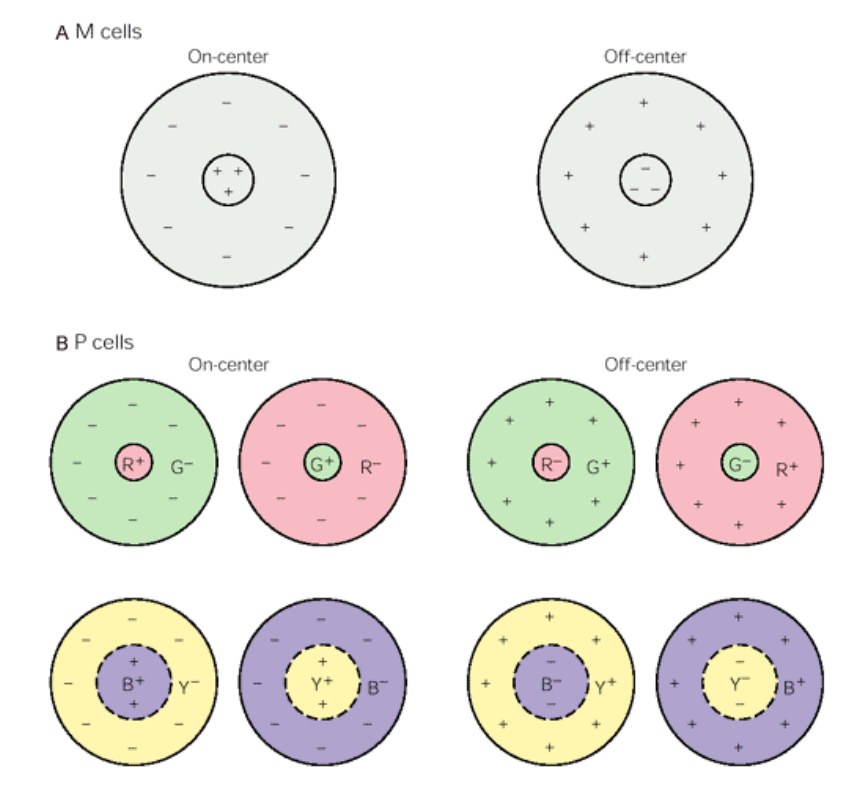
\includegraphics[width=0.5\textwidth]{images/DoG-RGB.png} 
                    \captionsetup{width=.8\linewidth}
                    \caption{\textbf{میدان گیرنده سلول های گانگلیونی.} 
                    این نمودار میدان های پذیرنده سلول های گانگلیونی 
                    M و P 
                    را نشان می دهد. عکس 
                    A 
                    سلول های 
                    M 
                    را با پیکربندی استاندارد روی مرکز و خارج از مرکز حساس به شدت نور نشان می دهد. عکس 
                    B 
                    سلول‌های 
                    P 
                    را با میدان‌های دریافتی مخالف رنگ برای تضادهای قرمز-سبز و آبی-زرد به تصویر می‌کشد که پاسخ‌های مرکز و خارج از مرکز آنها را به محرک‌های رنگی منعکس می‌کند.
                    }
                    \label{fig:part1-DoG-RGB}
                \end{figure}
                در  این قسمت ما از عملیات کانوولوشن با استفاده از فیلتر 
                DoG 
                بر روی یک تصویر به منظور بررسی تاثیر آن در برجسته سازی و بهبود ویژگی‌های بصری خاص که قابلیت‌های پردازشی سلول‌های گانگلیون 
                P 
                در شبکیه انسان را شبیه سازی می‌کند، استفاده کردیم.
                (شکل \ref{fig:part1-DoG-RGB-convolution})
                این فیلتر 
                DoG 
                رنگی، که برای تشخیص تضادهای رنگی و جزئیات مکانی طراحی شده است، به طور جداگانه بر روی کانال‌های قرمز و سبز تصویر اعمال شد. فرایند شامل تقویت نواحی که رنگ‌های مشخص در آنها غالب بود و سرکوب سایر نواحی می‌شد، که این امر تضاد کروماتیک مشاهده شده در سلول‌های 
                P 
                را تکرار می‌کند. نتایج این کانوولوشن نشان می‌دهد که چگونه برخی رنگ‌ها بیشتر برجسته می‌شوند، در حالی که برخی دیگر عقب‌تر می‌روند، و به طور مؤثر نشان می‌دهد که چگونه پردازش مشابه گانگلیون می‌تواند در سیستم‌های بصری مصنوعی برای اولویت‌بندی و تفکیک اطلاعات بصری بر اساس پویایی رنگ‌ها استفاده شود.

                \begin{figure}[!ht]
                    \centering
                    \includegraphics[width=0.6\textwidth]{plots/part1-DoG-RGB.pdf} 
                    \captionsetup{width=.7\linewidth}
                    \caption{\textbf{کاربرد کانولوشن فیلتر 
                    DoG
                    رنگی روی یک تصویر.} 
                    عکس سمت چپ تصویر اصلی را نشان می دهد، در حالی که عکس  سمت راست یا پایین نتایج را پس از اعمال فیلتر رنگی تفاوت گاوسی 
                    (DoG) 
                    روی کانال های قرمز و سبز نشان می دهند. همانطور که از شکل نیز پیداست، فیلتر توانسته است به خوبی بین روی تصویر اعمال شود. این نشان دهنده ظرفیت فیلتر برای افزایش و متمایز کردن ویژگی های خاص رنگ، تقلید از مخالفت رنگی سلول های گانگلیونی 
                    P 
                    در لایه های اولیه بینایی است.
                    }
                    \label{fig:part1-DoG-RGB-convolution}
                \end{figure}
\newpage
\chapter{روش های ارتباطی بین لایه های مختلف در شبکه های عصبی ضربه‌ای}
    \section{مقدمه}
    در این بخش از پروژه، هدف ما ساخت و پیاده‌سازی یک شبکه عصبی ضربه‌ای است که بتواند ویژگی های تکراری از تصاویر ورودی را پردازش، تحلیل و پیدا کند.شبکه‌های عصبی ضربه‌ای 
    (SNN) 
    نوعی از شبکه‌های عصبی مصنوعی هستند که الهام گرفته از شبکه‌های عصبی بیولوژیکی و نحوه عملکرد نورون‌های مغز می‌باشند. برخلاف شبکه‌های عصبی سنتی، نورون‌ها در 
    SNN 
    به جای تولید سیگنال‌های پیوسته، سیگنال‌های گسسته و ضربه‌ای تولید می‌کنند که به آن‌ها امکان می‌دهد تا اطلاعات را به شیوه‌ای کارآمدتر و با مصرف انرژی کمتر پردازش کنند.

    در این پروژه، شبکه عصبی ضربه‌ای ما از فیلترهای 
    DoG (\lr{Difference of Gaussian}) 
    برای کدگذاری اولیه تصاویر استفاده می‌کند. فیلترهای 
    DoG 
    به دلیل توانایی بالا در استخراج ویژگی‌های مهم از تصاویر، به عنوان ابزارهای اصلی در مراحل پیش‌پردازش انتخاب شده‌اند. در مرحله بعد، لایه‌های دیگری مانند 
    Max-Pooling 
    برای کاهش ابعاد و لایه‌های یادگیری بدون ناظر برای استخراج ویژگی‌های پیچیده‌تر به شبکه اضافه خواهند شد.

    شبکه عصبی ضربه‌ای طراحی شده در این پروژه با الهام از ساختارها و مکانیسم‌های معرفی شده در چارچوب 
    CoNeX 
    ساخته شده است. 
    CoNeX 
    یک چارچوب محاسباتی برای مدل‌سازی و شبیه‌سازی شبکه‌های عصبی ضربه‌ای با الهام از سیستم‌های عصبی بیولوژیکی است و ابزارهای مختلفی را برای پیاده‌سازی و ارزیابی این نوع شبکه‌ها فراهم می‌کند.
    
    در این شبکه عصبی ضربه‌ای، تصاویر ورودی ابتدا توسط فیلترهای DoG پردازش و کدگذاری می‌شوند. سپس، لایه‌های دیگری مانند 
    Max-Pooling 
    و لایه‌های یادگیری بدون ناظر به شبکه اضافه می‌شوند تا ویژگی‌های پیچیده‌تری از تصاویر استخراج شود. این شبکه عصبی ضربه‌ای سپس با استفاده از مجموعه‌ای از تصاویر طبیعی آموزش داده شده و نتایج حاصله تحلیل و بررسی می‌شود.
    
    هدف نهایی از این بخش، بررسی تأثیر پارامترهای مختلف فیلترها و لایه‌ها بر عملکرد شبکه و بهبود دقت در تشخیص و طبقه‌بندی تصاویر است. با انجام این مرحله، دانشجویان با مفاهیم و تکنیک‌های مختلف در طراحی و پیاده‌سازی شبکه‌های عصبی ضربه‌ای آشنا شده و توانایی‌های عملی خود را در این زمینه بهبود می‌بخشند.

    \section{معماری شبکه}
    معماری شبکه عصبی ضربه‌ای (Spiking Neural Network) که در این پروژه پیاده‌سازی شده است، شامل یک لایه ورودی، یک لایه خروجی و سیناپس‌های متصل‌کننده این دو لایه می‌باشد. این معماری با هدف پردازش و تحلیل تصاویر ورودی به صورت موثر و کارآمد طراحی شده است. در ادامه، به توضیح جزئیات هر یک از اجزای این معماری می‌پردازیم.

    \subsection*{لایه ورودی}
        لایه ورودی اولین بخش شبکه است که تصاویر را دریافت کرده و آنها را به ضربه‌های نورونی تبدیل می‌کند. فرآیند در این لایه شامل چند مرحله است:
        \begin{itemize}
            \item \textbf{تبدیل تصاویر به مقیاس خاکستری:} در ابتدا، تصاویر رنگی به تصاویر خاکستری تبدیل می‌شوند تا پردازش ساده‌تر و سریع‌تر انجام شود.
            \item \textbf{اعمال فیلتر 
            DoG:} 
            این فیلتر به منظور استخراج ویژگی‌های کلیدی از تصاویر به کار می‌رود. فیلتر 
            DoG 
            تفاوت بین دو تابع گوسی با مقیاس‌های مختلف را محاسبه می‌کند و به تشخیص لبه‌ها و جزئیات مهم کمک می‌کند.
            \item \textbf{نرمال‌سازی و تغییر اندازه:} تصاویر نرمال‌سازی شده و به ابعاد مناسب برای پردازش در شبکه تغییر اندازه داده می‌شوند.
            \item \textbf{مدل نورونی تجمیع و آتش نشتی:}  این مدل برای شبیه‌سازی رفتار نورون‌های بیولوژیکی استفاده می‌شود. نورون‌ها در این مدل با دریافت ورودی‌ها، بار الکتریکی را جمع‌آوری کرده و پس از رسیدن به یک آستانه مشخص، تخلیه می‌شوند و ضربه تولید می‌کنند.
            \item \textbf{کدگذاری ضربه‌های نورونی:} در نهایت، تصاویر به ضربه‌های نورونی تبدیل می‌شوند. این کدگذاری به شکل Time-to-First-Spike 
            انجام می‌شود که در آن شدت پیکسل‌ها به زمان تأخیر ضربه‌ها تبدیل می‌شود.
        \end{itemize}
    \subsection*{لایه خروجی} 
        لایه خروجی شامل گروهی از نورون‌ها است که مسئول پردازش و تحلیل نهایی ویژگی‌های استخراج شده از تصاویر هستند. ویژگی‌های اصلی این لایه عبارتند از:
        \begin{itemize}
            \item \textbf{مدل نورونی تجمیع و آتش نشتی:} 
            دقیقا همان مدلیست که در لایه اول استفاده شده است.
            \item \textbf{مکانیسم 
            KWTA (k-Winners-Take-All):}
            این مکانیسم برای محدود کردن تعداد نورون‌های فعال در هر لحظه استفاده می‌شود و به افزایش کارایی و دقت شبکه کمک می‌کند.
            \item \textbf{\lr{Spike Trace} و \lr{Homeostasis} :}  این ویژگی‌ها برای تنظیم فعالیت نورون‌ها و حفظ تعادل شبکه استفاده می‌شوند، به طوری که شبکه به طور پایدار عمل کند و از بیش‌فعالی یا کم‌فعالی نورون‌ها جلوگیری شود.
        \end{itemize}

    \subsection*{سیناپس ها}
        سیناپس‌ها اتصالاتی هستند که اطلاعات را بین لایه‌های ورودی و خروجی انتقال می‌دهند. در این شبکه، سیناپس‌ها از کانولوشن برای انتقال سیگنال‌ها و یادگیری استفاده می‌کنند. رفتار های کلیدی سیناپس‌ها عبارتند از:
        \begin{itemize}
            \item \textbf{نرمال سازی وزن ها\footnote{\lr{Weight Normalization:}}}  این فرآیند به تنظیم وزن‌های سیناپس‌ها کمک می‌کند تا سیگنال‌ها به طور متناسب و بهینه انتقال یابند.
            \item \textbf{\lr{Conv2dSTDP} :} این مکانیزم یادگیری بر پایه زمان‌بندی ضربه‌ها عمل می‌کند. اگر یک نورون پس از دیگری ضربه بزند، وزن سیناپسی بین آن‌ها تقویت یا تضعیف می‌شود. این مدل یادگیری را در پروژه های قبل به طور مفصل بررسی کردیم. در این شبکه، 
            STDP 
            به صورت کانولوشنی اعمال می‌شود که امکان یادگیری ویژگی‌های پیچیده را فراهم می‌کند.
            \item \textbf{مهار جانبی (\lr{Lateral Inhibition}): }
            این ویژگی به تنظیم فعالیت نورون‌ها در لایه خروجی کمک می‌کند، به طوری که فعالیت یک نورون می‌تواند فعالیت نورون‌های مجاور را مهار کند و از فعال شدن همزمان بیش از حد نورون‌ها جلوگیری کند.
        \end{itemize}

    \section{آموزش شبکه}
        در این پروژه از مجموعه داده‌های 
        \lr{Yale Faces} 
        برای آموزش و ارزیابی شبکه عصبی ضربه‌ای استفاده شده است. مجموعه داده‌های 
        \lr{Yale Faces} 
        یکی از مجموعه داده‌های شناخته شده و پرکاربرد در زمینه شناسایی و تشخیص چهره است. این مجموعه داده شامل تصاویر چهره افراد مختلف با حالات و شرایط نوری متفاوت می‌باشد. در شکل 
        \ref{fig:part2-sample-dataset}
        چند نمونه از این دیتاست آورده شده است.
        \paragraph*{مشخصات مجموعه داده \lr{Yale Faces}}
        \begin{itemize}
            \item \textbf{تعداد تصاویر:} مجموعه داده 
            \lr{Yale Faces} 
            شامل 165 تصویر از 
            15 
            فرد مختلف است. هر فرد در 
            11 
            حالت مختلف چهره عکاسی شده است که شامل حالت‌های مختلف نوری و حالات چهره (مانند لبخند زدن، چشم‌های بسته، و غیره) می‌شود.
            \item \textbf{ابعاد تصاویر:} تمامی تصاویر در این مجموعه داده به صورت سیاه و سفید با ابعاد
            ۱۰۰*۱۰۰
            انتخاب شده اند.
            \item \textbf{حالات چهره:} تمامی حالات چهره انتخاب شده، عادی و بدون حالت انتخاب شده‌اند.
        \end{itemize}


        \begin{figure}[!ht]
            \centering
            \includegraphics[width=0.8\textwidth]{plots/part2-sample-dataset.pdf} 
            \captionsetup{width=.7\linewidth}
            \caption{\textbf{چند نمونه تصویر از دیتاست اصلی} 
            }
            \label{fig:part2-sample-dataset}
        \end{figure}

        \subsection{پیش‌پردازش داده‌ها}
            برای آماده‌سازی داده‌ها برای ورود به شبکه عصبی ضربه‌ای، مجموعه داده 
            \lr{Yale Faces} 
            تحت چند مرحله پیش‌پردازش قرار گرفته است:
            \begin{itemize}
                \item \textbf{تبدیل به مقیاس خاکستری:} تصاویر رنگی موجود در مجموعه داده به تصاویر خاکستری تبدیل شده‌اند. این کار به منظور کاهش پیچیدگی و حجم محاسباتی پردازش تصاویر انجام شده است.
                \item \textbf{اعمال فیلتر 
                DoG :} به منظور استخراج ویژگی‌های کلیدی از تصاویر، فیلتر DoG 
                بر روی تصاویر اعمال شده است. این فیلتر به شناسایی لبه‌ها و جزئیات مهم در تصاویر کمک می‌کند.
                \item \textbf{نرمال‌سازی و تغییر اندازه:}
                 تصاویر نرمال‌سازی شده و به ابعاد مناسبی برای پردازش در شبکه 
                 (مانند 128x128 پیکسل) 
                 تغییر اندازه داده شده‌اند. این کار باعث می‌شود که تمامی تصاویر ورودی دارای ابعاد یکنواختی باشند و پردازش بهینه‌تر انجام شود.
                 \item \textbf{کدگذاری ضربه‌های نورونی:} تصاویر نرمال‌سازی شده و تغییر اندازه داده شده به ضربه‌های نورونی تبدیل شده‌اند. این کدگذاری به شکل Time-to-First-Spike 
                 انجام شده است که در آن شدت پیکسل‌ها به زمان تأخیر ضربه‌ها تبدیل می‌شود.
            \end{itemize}

        این مجموعه داده با توجه به تنوع حالات چهره و شرایط نوری مختلف، یک چالش مناسب برای ارزیابی و بهبود عملکرد شبکه عصبی ضربه‌ای فراهم می‌کند. استفاده از این داده‌ها به ما امکان می‌دهد تا کارایی و دقت شبکه را در شرایط مختلف بررسی کنیم و به بهبود معماری و روش‌های یادگیری شبکه بپردازیم.
        
        \subsection{آموزش شبکه}
            در این بخش از گزارش، به تحلیل و بررسی عملکرد شبکه عصبی ضربه‌ای 
            (SNN) مان
            که پیاده‌سازی شده است، می‌پردازیم. هدف از انجام این آزمایش‌ها، بررسی دقت و کارایی شبکه در پردازش و تشخیص ویژگی های تکراری تصاویر مجموعه داده است. همچنین، تحلیل عمیق‌تری از نحوه استخراج ویژگی‌ها توسط لایه کانولوشن و تأثیر پارامترهای مختلف بر عملکرد شبکه انجام می‌دهیم.
            
            ابتدا به تحلیل و بررسی نتایج حاصل از اولین آزمایش انجام شده توسط شبکه‌مان
            می‌پردازیم. هدف این آزمایش بررسی عملکرد شبکه در استخراج ویژگی‌های مهم از تصاویر ورودی با استفاده از لایه کانولوشن و تحلیل صفحه‌های ویژگی 
            (Feature Maps) 
            به دست آمده است. پارامترهای تنظیم شده برای این آزمایش شامل تعداد فیلترها، اندازه فیلترها، نرخ فعالیت و پارامترهای یادگیری است که به صورت زیر تعریف شده‌اند:
            \begin{multicols}{3}
                پارامتر های لایه ورودی:
                \begin{itemize}
                \item تعداد مراحل شبیه‌سازی: ۹۹۰
                \item پنجره زمانی ورودی: ۱۰
                \item طول لایه اول: ۱۰۰
                \item عرض لایه اول: ۱۰۰
                \item $\tau_{trace}$ لایه اول: ۴
                \item تعداد کانال های ورودی: ۱
                \end{itemize}
                
                \columnbreak
                
                پارامتر های لایه دوم:
                \begin{itemize}
                \item طول کرنل: ۱۱
                \item عرض کرنل: ۱۱
                \item تعداد صفحه های ویژگی: ۹
                \item طول لایه خروجی:  تفاضل طول لایه ورودی و کرنل به علاوه ۱
                \item عرض لایه خروجی:  تفاضل عرض لایه ورودی و کرنل به علاوه ۱
                \item آستانه ضربه زدن نورون ها: ۱۵
                \item $\tau$ نورون ها: ۳
                \item $v_{rest}$ نورون ها: ۵
                \item مقاومت نورون ها: ۱۰
                \item $tau_{trace}$ نورون ها: ۳
                \end{itemize}
                \columnbreak

                پارامتر های ساز و کار ها:
                \begin{itemize}
                \item k در kwta: ۱
                \item نرخ فعالیت: ۰.۲
                \item اندازه پنجره فعالیت: ۱۰
                \item نرخ بروزرسانی فعالیت: ۱
                \item ضریب وزن ها: ۳۰۰
                \item مقدار $A_{+}$ : ۲
                \item مقدار $A_{-}$ : ۱
                \item مقدار ضریب مهار جانبی: ۱۰۰
                \end{itemize}
                \end{multicols}

                مطابق شکل 
                \ref{fig:part2-exp1-extracted-features}
                صفحه های ویژگی به دست آمده از لایه کانولوشن، نشان‌دهنده الگوهای مختلفی است که فیلترهای کانولوشنی استخراج کرده‌اند. در این آزمایش، از
                9
                فیلتر کانولوشن با ابعاد 
                ۹*۹
                استفاده شده است. هر یک از صفحه‌های ویژگی به صورت یک ماتریس نمایش داده شده است که نشان‌دهنده وزن یادگرفته شده سیناپس بین نورون‌ها در پاسخ به ویژگی‌های مختلف تصویر ورودی است.

                در تصاویر صفحه های ویژگی ارائه شده، می‌توان مشاهده کرد که هر فیلتر به ویژگی‌های مختلفی از تصویر حساس است. برخی از فیلترها به لبه‌های عمودی، برخی به لبه‌های افقی و برخی به نواحی با شدت نور مختلف حساسیت نشان داده‌اند. این نشان می‌دهد که فیلترهای کانولوشن توانسته‌اند ویژگی‌های مهمی را از تصاویر ورودی استخراج کنند.

                \begin{figure}[!ht]
                    \centering
                    \includegraphics[width=0.8\textwidth]{plots/part2-exp1-extracted-features.pdf} 
                    \captionsetup{width=.9\linewidth}
                    \caption{\textbf{آزمایش اول: ویژگی های استخراج شده.} در آزمایش اول با یک سری پارامتر اولیه شروع می‌کنیم و رفته رفته پارامترها را بهبود می‌دهیم. مطابق شکل  هر تصویر نشان‌دهنده الگوهایی است که یک فیلتر خاص از تصویر ورودی استخراج کرده است. این صفحه‌ها نشان می‌دهند که فیلترها به لبه‌ها و نواحی با شدت نور مختلف حساسیت دارند و ویژگی‌های متنوعی از تصاویر ورودی را شناسایی می‌کنند. هر چند که بعضی ویژگی ها به خوبی استخراج شده اند، ولی هنوز شاهد ویژگی هایی هستیم که می‌توانند بهتر شوند.
                    }
                    \label{fig:part2-exp1-extracted-features}
                \end{figure}

                حال ویژگی های استخراج شده را، روی یک تصویر ورودی هم‌گشت می‌کنیم تا نتیجه استخراج ویژگی ها را مشاهده کنیم. به عنوان مثال، در شکل 
                \ref{fig:part2-exp1-output-last-iteration-single}
                مشاهده می‌کنیم که ویژگی شماره ۶ توانسته است لبه ها را به خوبی تشخیص دهد.

                \begin{figure}[!ht]
                    \centering
                    \includegraphics[width=0.8\textwidth]{plots/part2-exp1-output-last-iteration-single.pdf} 
                    \captionsetup{width=.9\linewidth}
                    \caption{\textbf{ هم‌گشت ویژگی های استخراج شده روی یک نمونه تصویر ورودی.}  این تصویر حاصل عملیات کانولوشن یکی از فیلترهای شبکه بر روی تصویر ورودی در آخرین تکرار آموزش است. نواحی سفید نشان‌دهنده نورون‌های فعال شده هستند که نشان می‌دهد فیلتر کانولوشنی توانسته ویژگی‌های خاصی از تصویر ورودی را شناسایی و استخراج کند. این خروجی نشان‌دهنده کارایی فیلترهای کانولوشنی در شناسایی و پردازش الگوهای موجود در تصویر است.
                    }
                    \label{fig:part2-exp1-output-last-iteration-single}
                \end{figure}

                برای بررسی دقیق‌تر و بهبود بیشتر عملکرد شبکه، به آزمایش دوم با پارامترهای جدید می‌پردازیم. در این آزمایش، پارامترهایی نظیر نرخ فعالیت، و تنظیمات کرنل‌ها تغییر یافته‌اند تا تاثیر این تغییرات بر عملکرد کلی شبکه مورد ارزیابی قرار گیرد. 
            
                همانطور که در شکل 
                \ref{fig:part2-exp2-extracted-features}
                مشاهده می‌کنید، با افزایش 
                $\tau_s$، 
                و همچنین پارامتر های 
                $A_{+}$ و $A_{-}$ 
                شاهد بهبود هایی در صفحه های ویژگی پیدا شده هستیم. هرچند هنوز نیز می‌توان انتظار بهبود بیشتری نیز داشت. به عنوان مثال، چهار ویژگی از صفحات ویژگی مشابه یکدیگر هستند و یک چیز را یادگرفته‌اند. 

                \begin{figure}[!ht]
                    \centering
                    \includegraphics[width=0.8\textwidth]{plots/part2-exp2-extracted-features.pdf} 
                    \captionsetup{width=.9\linewidth}
                    \caption{\textbf{ صفحه های ویژگی به دست آمده از فیلترهای کانولوشن در لایه دوم با پارامترهای بهبود یافته: تنظیم پارامتر $\tau_s$. } در آزمایش دوم، مقدار 
                    $tau_s$ را بیشتر کرده و مطابق شکل ملاحظه می‌کنیم که ویژگی های بهتری استخراج شده است.
                    افزایش مقدار 
                    $\tau_s$ 
                    به 10، زمان پایداری سیگنال‌ها را افزایش می‌دهد که منجر به استخراج بهتر ویژگی‌های زمانی می‌شود.
                    }
                    \label{fig:part2-exp2-extracted-features}
                \end{figure}

                مطابق شکل
                \ref{fig:part2-exp2-output-last-duration} 
                می‌توان مشاهده کرد که نورون‌های مختلف در عمق‌های مختلف شبکه به ویژگی‌های خاصی از تصویر ورودی واکنش نشان داده‌اند. نواحی سفید نشان‌دهنده نورون‌های فعال شده هستند که نشان می‌دهد فیلتر کانولوشنی توانسته ویژگی‌های خاصی از تصویر ورودی را شناسایی و استخراج کند. فیلترهای کانولوشنی توانسته‌اند ویژگی‌های متنوعی از تصاویر ورودی را استخراج کنند که نشان‌دهنده قدرت شبکه در تشخیص الگوهای مختلف است. برخی از صفحه‌های ویژگی و خروجی‌های نهایی وضوح کمتری دارند و نشان‌دهنده این است که ممکن است برخی از فیلترها نیاز به تنظیمات بیشتری داشته باشند.

                \begin{figure}[!ht]
                    \centering
                    \includegraphics[width=0.8\textwidth]{plots/part2-exp2-output-last-duration.pdf} 
                    \captionsetup{width=.9\linewidth}
                    \caption{\textbf{ خروجی شبکه در آخرین پنجره زمانی برای هر یک از   فیلترهای کانولوشن: تنظیم پارامتر $\tau_s$. } مطابق شکل ملاحظه می‌کنیم که شبکه توانسته است تعداد خوبی از ویژگی های تصاویر را یاد بگیرد به طوری که بعضی از ویژگی های چهره مانند فرم کلی در خروجی ها مشهود است. نواحی سفید نشان‌دهنده نورون‌های فعال شده هستند که نشان می‌دهند فیلترهای کانولوشنی توانسته‌اند ویژگی‌های خاصی از تصویر ورودی را شناسایی و استخراج کنند. این خروجی‌ها نشان‌دهنده کارایی فیلترهای کانولوشنی در شناسایی و پردازش الگوهای موجود در تصویر هستند. با افزایش $\tau_s$، شبکه توانسته است الگوهای بهتری و متنوع‌تری را از تصاویر استخراج کند که بهبود قابل توجهی در دقت شناسایی ویژگی‌های کلی را نشان می‌دهد.
                    }
                    \label{fig:part2-exp2-output-last-duration}
                \end{figure}

                در آخر، به بررسی پارامتر های 
                $A_{plus}$ و $A_{minus}$ 
                می‌پردازیم. این دو پارامتر از مهم ترین پارامتر های شبکه هستند چرا که مستقیما روی یادگیری شبکه تاثیر دارند. مطابق  شکل 
                \ref{fig:part2-exp3-extracted-features} 
                مشاهده می‌کنیم که تنظیم درست این پارامتر ها می‌تواند ویژگی های استخراج شده را به شدت بهبود دهد به طوری که تنوع ویژگی های پیدا شده افزایش یافته است.

                \begin{figure}[!ht]
                    \centering
                    \includegraphics[width=0.8\textwidth]{plots/part2-exp3-extracted-features.pdf} 
                    \captionsetup{width=.9\linewidth}
                    \caption{\textbf{  صفحه های ویژگی به دست آمده از فیلترهای کانولوشن در لایه دوم با پارامترهای بهبود یافته: تنظیم پارامتر های یادگیری.}  هر تصویر نشان‌دهنده الگوهایی است که یک فیلتر خاص از تصویر ورودی استخراج کرده است. مشاهده می‌کنیم که تنظیم درست پارمتر های یادگیری
                    ($A_{plus}$ و $A_{minus}$) 
                    توانسته است به خوبی ویژگی های مختلف را استخراج کند. 
                    این صفحه ها نشان می‌دهند که فیلترها به لبه‌ها و نواحی با شدت نور مختلف حساسیت دارند و ویژگی‌های متنوع‌تری از تصاویر ورودی را شناسایی می‌کنند. پارامترهای استفاده شده در این آزمایش در قسمت بالا سمت راست تصویر آورده شده‌اند.
                    }
                    \label{fig:part2-exp3-extracted-features}
                \end{figure}

                در شکل 
                \ref{fig:part2-exp3-output-last-duration}
                می‌توان مشاهده کرد که نورون‌های مختلف در عمق‌های مختلف شبکه به ویژگی‌های خاصی از تصویر ورودی واکنش نشان داده‌اند. نواحی سفید نشان‌دهنده نورون‌های فعال شده هستند که نشان می‌دهد فیلتر کانولوشنی توانسته ویژگی‌های خاصی از تصویر ورودی را شناسایی و استخراج کند. در یکی از تصاویر، صورت به خوبی تشخیص داده شده است که نشان‌دهنده بهبود قابل توجه دقت و کارایی شبکه است.

                \begin{figure}[!ht]
                    \centering
                    \includegraphics[width=0.8\textwidth]{plots/part2-exp3-output-last-duration.pdf} 
                    \captionsetup{width=.9\linewidth}
                    \caption{\textbf{ خروجی شبکه در آخرین پنجره زمانی برای هر یک از فیلترهای کانولوشن: تنظیم پارامتر های یادگیری. } مطابق شکل ملاحظه می‌کنیم که شبکه توانسته است تعداد بیشتری از ویژگی های تصاویر را یاد بگیرد به طوری که بعضی از ویژگی های چهره مانند فرم کلی یا خطوط عمودی و افقی صورت و همچنین جای چشم ها در خروجی ها مشهود است. نواحی سفید نشان‌دهنده نورون‌های فعال شده هستند که نشان می‌دهد فیلتر کانولوشنی توانسته ویژگی‌های خاصی از تصویر ورودی را شناسایی و استخراج کند. در یکی از تصاویر، صورت به خوبی تشخیص داده شده است که نشان‌دهنده بهبود قابل توجه دقت و کارایی شبکه است.
                    }
                    \label{fig:part2-exp3-output-last-duration}
                \end{figure}

                در شکل 
                \ref{fig:part2-exp3-conv-feature-single}
                نیز نتیجه هم‌گشت یکی از فیلتر های آزمایش سوم بر روی یک نمونه تصویر ورودی آمده است. مطابق شکل ملاحظه می‌کنیم که نسبت به آزمایش قبل نتیجه بهتر است.

                \begin{figure}[!ht]
                    \centering
                    \includegraphics[width=0.8\textwidth]{plots/part2-exp3-conv-feature-single.pdf} 
                    \captionsetup{width=.9\linewidth}
                    \caption{\textbf{ ویژگی های استخراج شده روی یک نمونه تصویر: تنظیم پارامتر های یادگیری. } مطابق شکل ملاحظه می‌کنیم که در این آزمایش با تنظیم پارامتر های گفته شده، ویژگی های استخراج شده نیز بهبود یافتند و تصویر هم‌گشت شده از یک نمونه تصویر دارای دقت بیشتری است.
                    }
                    \label{fig:part2-exp3-conv-feature-single}
                \end{figure}

                حال به بررسی تأثیر کاهش اندازه کرنل‌های کانولوشن بر عملکرد شبکه
                می‌پردازیم. اندازه کرنل‌ها نقش مهمی در فرآیند استخراج ویژگی‌های مختلف از تصاویر ورودی دارند. کاهش اندازه کرنل ممکن است به شبکه کمک کند تا جزئیات دقیق‌تری از تصاویر را استخراج کند و در عین حال پیچیدگی محاسباتی را کاهش دهد. هدف از این آزمایش، بررسی تأثیر تغییرات در اندازه کرنل بر وضوح و تنوع صفحه های ویژگی 
                و کارایی کلی شبکه در شناسایی و طبقه‌بندی الگوهای موجود در تصاویر ورودی است. با انجام این آزمایش، به دنبال یافتن اندازه بهینه کرنل برای بهبود دقت و کارایی شبکه هستیم.

                تصاویر صفحه‌های ویژگی به دست آمده از فیلترهای کانولوشن در لایه دوم شبکه، نشان‌دهنده الگوهای مختلفی است که فیلترها از تصویر ورودی استخراج کرده‌اند. در این آزمایش از
                9
                فیلتر کانولوشن با ابعاد 
                5*5
                استفاده شده است. هر یک از صفحه‌های ویژگی به صورت ماتریسی نمایش داده شده‌اند که شدت فعالیت نورون‌ها را در پاسخ به ویژگی‌های مختلف تصویر ورودی نشان می‌دهد. مطابق شکل 
                \ref{fig:part2-exp4-extracted-features-decrease-size}
                صفحه های ویژگی به دست آمده از فیلترهای کانولوشن در لایه دوم شبکه با اندازه کرنل کاهش یافته به 
                ۵*۵
                آمده است. هر تصویر نشان‌دهنده الگوهایی است که یک فیلتر خاص از تصویر ورودی استخراج کرده است. این نقشه‌ها نشان می‌دهند که فیلترها به لبه‌ها و نواحی با شدت نور مختلف حساسیت دارند و ویژگی‌های متنوع‌تری از تصاویر ورودی را شناسایی می‌کنند.

                \begin{figure}[!ht]
                    \centering
                    \includegraphics[width=0.8\textwidth]{plots/part2-exp4-extracted-features-decrease-size.pdf} 
                    \captionsetup{width=.9\linewidth}
                    \caption{\textbf{ صفحه های ویژگی به دست آمده از فیلترهای کانولوشن در لایه دوم با پارامترهای بهبود یافته: کاهش ابعاد صفحات ویژگی}  در تصاویر صفحه های ویژگی، می‌توان مشاهده کرد که هر فیلتر به ویژگی‌های مختلفی از تصویر حساس است. برخی از فیلترها به لبه‌های عمودی، برخی به لبه‌های افقی و برخی به نواحی با شدت نور مختلف حساسیت نشان داده‌اند. این نشان می‌دهد که فیلترهای کانولوشن با اندازه کوچک‌تر نیز توانسته‌اند ویژگی‌های مهمی را از تصاویر ورودی استخراج کنند. با این حال، وضوح برخی از صفحه های ویژگی نسبت به آزمایش‌های قبلی کاهش یافته است که ممکن است به دلیل اندازه کوچک‌تر کرنل باشد.
                    }
                    \label{fig:part2-exp4-extracted-features-decrease-size}
                \end{figure}

                مطابق شکل 
                \ref{fig:part2-exp4-output-last-duration}
                خروجی شبکه در آخرین پنجره زمانی برای هر یک از عمق‌های مختلف فیلترهای کانولوشن با اندازه کرنل کاهش یافته به 
                ۵*۵ 
                آمده است.
                نواحی سفید نشان‌دهنده نورون‌های فعال شده هستند که نشان می‌دهند فیلترهای کانولوشنی توانسته‌اند ویژگی‌های خاصی از تصویر ورودی را شناسایی و استخراج کنند.

                \begin{figure}[!ht]
                    \centering
                    \includegraphics[width=0.8\textwidth]{plots/part2-exp4-output-last-duration.pdf} 
                    \captionsetup{width=.9\linewidth}
                    \caption{\textbf{ خروجی شبکه در آخرین پنجره زمانی برای هر یک از فیلترهای کانولوشن: کاهش ابعاد صفحات ویژگی. } در این تصاویر می‌توان مشاهده کرد که نورون‌های مختلف در عمق‌های مختلف شبکه به ویژگی‌های خاصی از تصویر ورودی واکنش نشان داده‌اند.(
                        مانند لبه های عمودی، افقی
                    ) نواحی سفید نشان‌دهنده نورون‌های فعال شده هستند که نشان می‌دهد فیلتر کانولوشنی توانسته ویژگی‌های خاصی از تصویر ورودی را شناسایی و استخراج کند. با این حال، وضوح و تعداد نورون‌های فعال شده در برخی از عمق‌ها نسبت به آزمایش‌های قبلی کمتر است.
                    }
                    \label{fig:part2-exp4-output-last-duration}
                \end{figure}

                در شکل 
                \ref{fig:part2-exp4-conv-feature-single}
                نیز عملیات هم‌گشت روی یک نمونه تصویر ورودی انجام شده است. مطابق شکل ملاحظه می‌کنیم که کرنل کوچک تر و با پارامتر های بهبود یافته به خوبی توانسته است ویژگی هایی را از ورودی استخراج کند.

                \begin{figure}[!ht]
                    \centering
                    \includegraphics[width=0.8\textwidth]{plots/part2-exp4-conv-feature-single.pdf} 
                    \captionsetup{width=.9\linewidth}
                    \caption{\textbf{ ویژگی های استخراج شده روی یک نمونه تصویر: کاهش ابعاد صفحات ویژگی. } مطابق شکل ملاحظه می‌کنیم که در این آزمایش با تنظیم پارامتر های گفته شده، ویژگی های استخراج شده نیز بهبود یافتند و تصویر هم‌گشت شده از یک نمونه تصویر دارای دقت خوبی است.
                    }
                    \label{fig:part2-exp4-conv-feature-single}
                \end{figure}

                حال به بررسی تأثیر افزایش اندازه کرنل‌های کانولوشن بر عملکرد شبکه
                می‌پردازیم. افزایش اندازه کرنل‌ها ممکن است به شبکه کمک کند تا ویژگی‌های بیشتری را از نواحی بزرگ‌تری از تصاویر استخراج کند، که می‌تواند منجر به بهبود دقت در شناسایی الگوهای پیچیده‌تر شود. هدف از این آزمایش، بررسی تغییرات در وضوح و تنوع صفحات ویژگی
                و کارایی کلی شبکه در شناسایی و طبقه‌بندی الگوهای موجود در تصاویر ورودی با افزایش اندازه کرنل‌ها است. با انجام این آزمایش، به دنبال یافتن اندازه بهینه کرنل برای بهبود دقت و کارایی شبکه هستیم.

                مطابق شکل 
                \ref{fig:part2-exp5-extracted-features-increase-size}
                مشاهده می‌کنیم که با افزایش اندازه صفحهات ویژگی، ویژگی های استخراج شده از تصاویر ورودی نیز نسبتا بزرگتر شده اند. هر چند برخی وزن ها به طور کامل موفق به یادگیری نشده اند، ولی نتیجه کلی مطلوب است.

                در شکل 
                \ref{fig:part2-exp5-output-last-duration}
                نیز خروجی این تصاویر در لایه آخر که حاصل کانولوشن لایه اول در صفحات ویژگی هاست آمده است.

                \begin{figure}[!ht]
                    \centering
                    \includegraphics[width=0.8\textwidth]{plots/part2-exp5-extracted-features-increase-size.pdf} 
                    \captionsetup{width=\linewidth}
                    \caption{\textbf{ صفحه های ویژگی به دست آمده از فیلترهای کانولوشن در لایه دوم با پارامترهای بهبود یافته: افزایش ابعاد صفحات ویژگی.}  در تصاویر صفحه های ویژگی، می‌توان مشاهده کرد که هر فیلتر ویژگی‌های مختلف بزرگتری از تصویر را یادگرفته است. افزایش اندازه کرنل منجر به شناسایی الگوهای بزرگ‌تر و پیچیده‌تر شده است. بعضی از صفحه های ویژگی وضوح بالاتری دارند و الگوهای بیشتری را نشان می‌دهند که این نشان‌دهنده توانایی بالای شبکه در شناسایی جزئیات پیچیده‌تر تصاویر است. هر چند بعضی از صفحات نیز موفق به یادگیری کامل الگو ها نشده اند. نکته مهمی که هنگام افزایش اندازه صفحات ویژگی باید توجه داشت، این موضوع است که پارمتر ساز و کار مهار جانبی نیز باید تغییر کند. 
                    این فرایند برای حفظ تعادل فعالیت نورون‌ها و جلوگیری از فعال شدن بیش از حد آنها مهم است. با افزایش اندازه کرنل، تعداد نورون‌های فعال شده افزایش می‌یابد، بنابراین برای جلوگیری از فعالیت بیش از حد و حفظ تعادل، پارامتر مهار جانبی نیز باید تغییر کند.
                    }
                    \label{fig:part2-exp5-extracted-features-increase-size}
                \end{figure}
                
                \begin{figure}[!ht]
                    \centering
                    \includegraphics[width=0.8\textwidth]{plots/part2-exp5-output-last-duration.pdf} 
                    \captionsetup{width=.9\linewidth}
                    \caption{\textbf{ خروجی شبکه در آخرین پنجره زمانی برای هر یک از فیلترهای کانولوشن: افزایش ابعاد صفحات ویژگی. } از آنجا که ابعاد کرنل بزرگتر شده است، در این تصاویر می‌توان مشاهده کرد که نورون‌های مختلف در عمق‌های مختلف شبکه به ویژگی‌های کلی تری از تصویر ورودی واکنش نشان داده‌اند، مانند فرم کلی صورت، محل قرار گیری چشم ها، موی سر یا بینی و اجزای دیگر صورت. 
                    }
                    \label{fig:part2-exp5-output-last-duration}
                \end{figure}
    
                \clearpage
    
    \section*{نتیجه گیری}
        در این پروژه، ما به بررسی و شبیه‌سازی پردازش اولیه تصاویر در سیستم بینایی انسان پرداختیم. با استفاده از فیلترهای تفاضل گاوسی 
        (DoG) 
        و گبور، موفق به شبیه‌سازی مکانیسم‌های پردازش اولیه در شبکیه و قشر بینایی اولیه
        شدیم. این فیلترها توانستند ویژگی‌های بصری مهمی مانند لبه‌ها و کنتراست‌ها را برجسته کرده و به شناسایی و تفسیر بهتر این ویژگی‌ها کمک کنند.

        استفاده از فیلترهای 
        DoG 
        و گبور نشان داد که چگونه می‌توان از مدل‌های محاسباتی برای تقلید از عملکرد بیولوژیکی سیستم بینایی استفاده کرد. نتایج حاصل از این شبیه‌سازی‌ها نشان داد که پیش‌پردازش تصاویر با این فیلترها می‌تواند به بهبود فرآیندهای کدگذاری عصبی و پردازش اطلاعات بصری منجر شود.
        
        همچنین در این پروژه به اهمیت نحوه کدگذاری عصبی ضربه‌ای 
        در پردازش اطلاعات بصری اشاره کردیم و نشان دادیم که چگونه این روش می‌تواند با استفاده از فیلترهای مناسب، کارایی و دقت پردازش‌های نورونی را افزایش دهد.
        
        در مجموع، این پروژه به درک بهتر از مکانیسم‌های پردازش اولیه در سیستم بینایی کمک کرد و نشان داد که چگونه می‌توان از مدل‌های محاسباتی برای مطالعه و تحلیل فرآیندهای پیچیده بیولوژیکی استفاده کرد.
\newpage
% \include{part3.tex}

%%%%%%%%%%%%%%%%%%%%%%%%%%% Bibliography section %%%%%%%%%%%%%%%%%%%%%%%%%%%
\begin{thebibliography}{1}
    \bibitem{textbook}
        \begin{latin}
            Computational Neuroscience Course, School of computer science, University of Tehran
        \end{latin}
    \bibitem{PymoNNtorch}
        \begin{latin}
            PymoNNtorchPytorch-adapted version of PymoNNto
        \end{latin}
    \bibitem{Neuronal-Dynamics}
        \begin{latin}
            \href{https://neuronaldynamics.epfl.ch/online/Ch12.S3.html}{Neuronal Dynamics, Wulfram Gerstner, Werner M. Kistler, Richard Naud and Liam Paninski
            }
        \end{latin}
    \bibitem{Lateral-inhibition-wikipedia}
        \begin{latin}
            Lateral inhibition. Wikipedia
            [\href{https://en.wikipedia.org/wiki/Lateral_inhibition}{Link}]
        \end{latin}
    \bibitem{Unsupervised-Learning-Lateral-Inhibition}
        \begin{latin}
            \href{https://infoscience.epfl.ch/record/232675?v=pdf}{Unsupervised Learning of Phase-Change-Based Neuromorphic Systems. Wozniak, Stanislaw Andrzej
            }
        \end{latin}
    % \bibitem{Poisson-Distribution-Wikipedia}
    %     \begin{latin}
    %         Poisson Distribution. Wikipedia
    %         [\href{https://en.wikipedia.org/wiki/Poisson_distribution}{Link}]
    %     \end{latin}
    % \bibitem{STDP-Wikipedia}
    %     \begin{latin}
    %         Spike-timing-dependent plasticity. Wikipedia
    %         [\href{https://en.wikipedia.org/wiki/Spike-timing-dependent_plasticity}{Link}]
    %     \end{latin}
    \end{thebibliography}
\end{document}
